\documentclass{bbawslides}

\usepackage[TS1, T1]{fontenc}
\usepackage{ifthen}

\usepackage[a4paper]{hyperref}
\rotateheaderstrue	%%-- otherwise seminar does strange things
\usepackage{url}

\usepackage[ngerman]{babel}
\usepackage[babel]{csquotes}
\usepackage[autoplay]{animate}
\usepackage{graphicx}
\usepackage{numprint}
\npthousandsep{~}\npthousandthpartsep{}\npdecimalsign{,}

\DeclareTextSymbol{\textlongs}{TS1}{115} 
\DeclareTextSymbolDefault{\textlongs}{TS1}


\begin{document}
\providecommand{\Title}{}


\begin{bbawtitle}[Praktische Probleme des OCR-Trainings mit synthetischen Daten]
  \vspace*{2em}%
  Kay-Michael Würzner\\[-.25em]%
  \textcolor{urlColor}{\texttt{{\small wuerzner@bbaw.de}}}
  \\[0.5em]
  {\small Gemeinsame Arbeit mit Ehud Alexander Avner und Matthias Boenig}
  \\[1.5em]
  {\footnotesize{%
    OCR-Entwicklerworkshop an der Berlin-Brandenburgischen Akademie der Wissenschaften\\%
    28. September 2017\\%
  }}
\end{bbawtitle}
\slideStyleFrame

\renewcommand{\footerText}{\tiny 28. September 2017, OCR-Entwicklerworkshop, BBAW}

%----------------------------------------------------------------------------------------------
% Outline
%----------------------------------------------------------------------------------------------
\begin{bbawslide}{Übersicht}
  \vspace*{7mm}%
  \centerslidestrue%
  \begin{itemize}
    \item Einleitung
    \begin{itemize}\small
      \item Was ist synthetisches Training?
      \item Wozu braucht man das?
    \end{itemize}
    \item Technische Aspekte
    \begin{itemize}\small
      \item Font-Rendering
      \item Schriftarten
      \item Unicode
      \item Volltexte
    \end{itemize}
    \item Experimente
    \begin{itemize}\small
      \item Hebräisch mit Nikkud
      \item Schreibmaschinenschrift
    \end{itemize}
  \end{itemize}
\end{bbawslide}

\begin{bbawpart}{\Large\bf Einleitung}
\end{bbawpart}

\begin{bbawslide}{Was ist synthetisches Training?}
  \vspace*{7mm}%
  \centerslidestrue%
  \begin{itemize}
    \item Text-Bild Alignierung als Grundlage jeden OCR-Trainings
    \begin{itemize}
      \item Zeilen- oder Glyphenebene
      \item hoher manueller Aufwand
      \item hohe Fehleranfälligkeit
    \end{itemize}
  \end{itemize}
  \begin{center}
    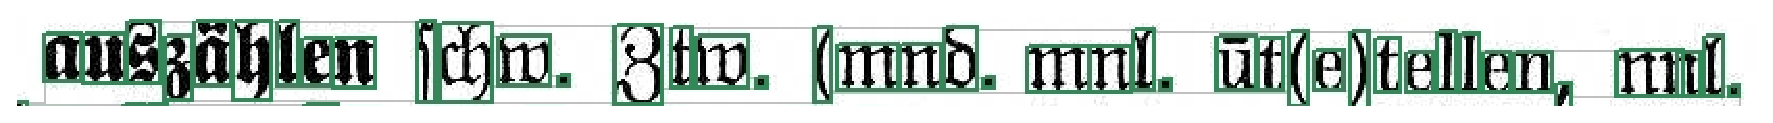
\epsfig{file=figures/align.eps,width=\textwidth}
  \end{center}
  \begin{itemize}
    \item Qualität der resultierenden Modelle abhängig von \textbf{Passung} und \textbf{Umfang} des Trainingsmaterials
    \item für die meisten Anwendungsszenarien: \textbf{keine} geeigneten Modelle und damit \textbf{schmutzige} OCR
  \end{itemize}
\end{bbawslide}

\begin{bbawslide}{Was ist synthetisches Training?}
  \vspace*{7mm}%
  \centerslidestrue%
    Training auf Basis von \textbf{maschinell generiertem} Trainingsmaterial
    \begin{enumerate}
      \item Font-Rendering-Engine
      \item Font (digitale Fassung einer Schriftart)
      \item Text
    \end{enumerate}
    \begin{center}
      \begin{tabular}{llc}
        \textbf{Text} & \textbf{Font} & \textbf{Bild} \\
         & Sans & \begin{minipage}{0.25\textwidth}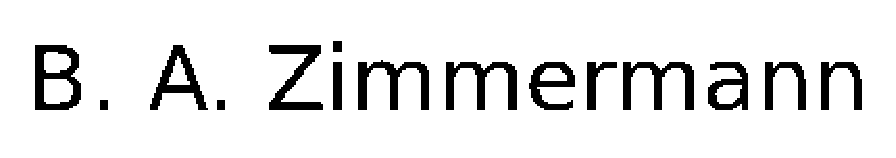
\epsfig{file=figures/ex_sans.eps,width=\textwidth}\end{minipage} \\
        & Times & \begin{minipage}{0.25\textwidth}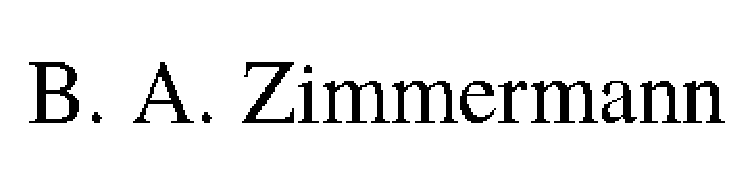
\epsfig{file=figures/ex_times.eps,width=\textwidth}\end{minipage}\\
         B. A. Zimmermann & Claudius & \begin{minipage}{0.25\textwidth}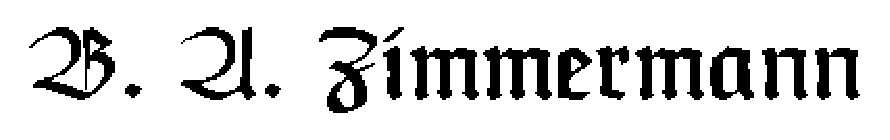
\epsfig{file=figures/ex_claudius.eps,width=\textwidth}\end{minipage} \\
         & Typenoksidi & \begin{minipage}{0.25\textwidth}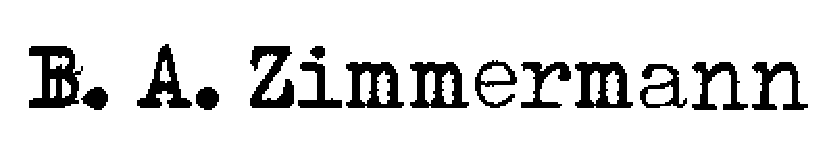
\epsfig{file=figures/ex_typenoksidi.eps,width=\textwidth}\end{minipage} \\
         & Typenoksidi & \begin{minipage}{0.25\textwidth}
\epsfig{file=figures/ex_typenoksidi_degr.eps,width=\textwidth}\end{minipage} \\
      \end{tabular}
    \end{center}
\end{bbawslide}

\begin{bbawslide}{Wozu braucht man das?}
  \vspace*{7mm}%
  \centerslidestrue%
  \begin{itemize}
    \item praktisch unbegrenzte Mengen an Trainingsmaterial generierbar
    \item Standardlösung für OCR-Training in \texttt{Tesseract 4}
    \begin{itemize}\small
       \item Zitat: \enquote{400000 textlines spanning about 4500 fonts}
       \item mglw. sogar einzige Möglichkeit des Trainings?
    \end{itemize}
    \item Utilisierung manuell transkribierter Texte für OCR-Training (z.B. DTA)
    \item Kombination mit realen Trainingsdaten möglich
    \item bisher keine (systematische) Auseinandersetzung mit den einzelnen Parametern vor dem Hintergrund des OCR-Ergebnisses von gedrucktem Text
  \end{itemize}
\end{bbawslide}

\begin{bbawpart}{\Large\bf Technische Aspekte}
\end{bbawpart}

\begin{bbawslide}{Font Rendering}
  \vspace*{7mm}%
  \centerslidestrue%
  \begin{itemize}
    \item
  \end{itemize}
\end{bbawslide}

\begin{bbawslide}{Schriftarten}
  \vspace*{7mm}%
  \centerslidestrue%
  \begin{itemize}
    \item
  \end{itemize}
\end{bbawslide}

\begin{bbawslide}{Unicode}
  \vspace*{7mm}%
  \centerslidestrue%
  \begin{itemize}
    \item
  \end{itemize}
\end{bbawslide}

\begin{bbawslide}{Volltexte}
  \vspace*{7mm}%
  \centerslidestrue%
  \begin{itemize}
    \item
  \end{itemize}
\end{bbawslide}

\begin{bbawpart}{\Large\bf Experimente}
\end{bbawpart}

\begin{bbawslide}{Experimente}
  \vspace*{7mm}%
  \centerslidestrue%
  \begin{description}
    \item[Ziel:] Ausloten der Potenziale des synthetischen Trainings in Kontexten ohne ausreichend vorhandenes reales Trainingsmaterial und mit erschwerten Bedingungen
    \item[Methode:] $~$
      \begin{itemize}
        \item Fontauswahl
        \item Generierung von Zeilenimages (unter verschiedenen Bedingungen) mit Hilfe von \texttt{OCRopus} und \texttt{Ketos}
        \begin{description}
          \item[$\rightarrow$] nur binärcodierte Bilder
        \end{description}
        \item Training von \texttt{OCRopus}- bzw. \texttt{CLSTM}- Modellen
        \item Evaluierung
      \end{itemize}
  \end{description}
\end{bbawslide}

\begin{bbawslide}{Experiment 1: Hebräisch mit Nikkud}
  \vspace*{7mm}%
  \centerslidestrue%
  \begin{itemize}
    \item Hebräisch
    \begin{itemize}\small
      \item alphabetische Sprache mit 22 Buchstaben
      \item keine \textbf{Vokale}
    \end{itemize}
    \item Nikkud (\enquote{Punkte, Punktierung})
    \begin{itemize}\small
      \item verschiedene Diakritika (über, unter und \textbf{innerhalb} von Buchstaben)
      \item Explifizierung von Vokalen und Konsonantenalternation
    \end{itemize}
    \item Aufwand der manuellen Transkription \textbf{horrend}
    \item Texte insbesondere aus dem Bereich Lyrik und Drama aber auch Lexika
    \item Vorarbeiten mit Tesseract 3 (\url{https://www.cs.bgu.ac.il/~elhadad/hocr/})
  \end{itemize}
\end{bbawslide}

\begin{bbawslide}{Experiment 1: Hebräisch mit Nikkud}
  \vspace*{3mm}%
  \centerslidestrue%
  \textbf{Beispiele:}
  \begin{center}
    \begin{tabular}{cc}
      \begin{minipage}{0.35\textwidth}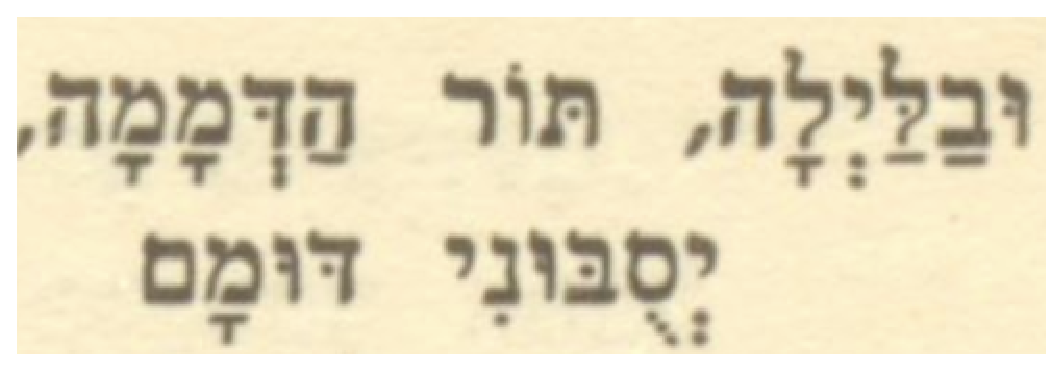
\epsfig{file=figures/ex_hebrew1.eps,width=\textwidth}\end{minipage}
      &
      \begin{minipage}{0.35\textwidth}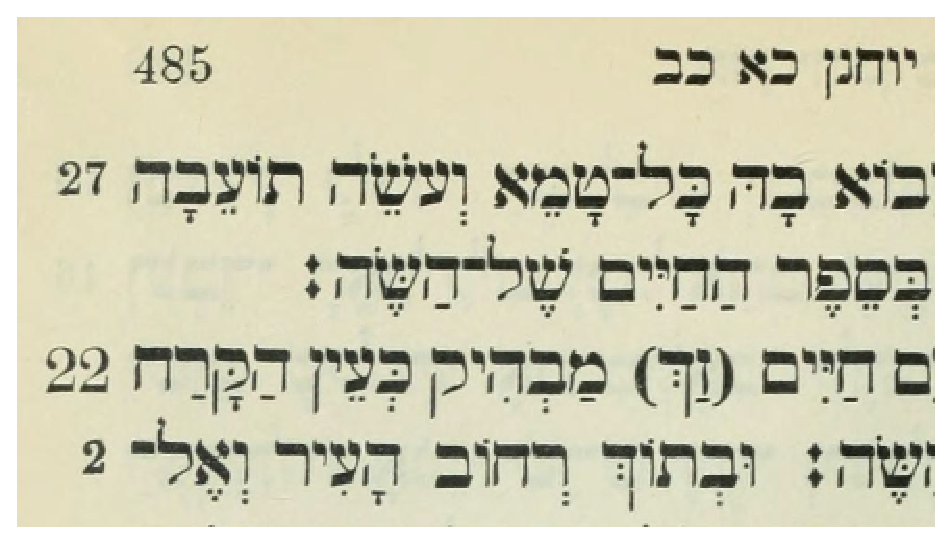
\epsfig{file=figures/ex_hebrew2.eps,width=\textwidth}\end{minipage}
    \end{tabular}\\[2ex]
    \begin{tabular}{cc}
      \begin{minipage}{0.5\textwidth}
\epsfig{file=figures/ex_hebrew5.eps,width=\textwidth}\end{minipage}
      &
      \begin{minipage}{0.5\textwidth}
\epsfig{file=figures/ex_hebrew4.eps,width=\textwidth}\end{minipage}
    \end{tabular}
  \end{center}
\end{bbawslide}

\begin{bbawslide}{Experiment 1: Hebräisch mit Nikkud}
  \vspace*{7mm}%
  \centerslidestrue%
  \textbf{Vorgehen:}
  \begin{itemize}
    \item manuelle Erfassung von zwei Seiten für Testzwecke (Text plus Layout, aligniert)
    \item Fontauswahl
    \begin{itemize}
      \item wenige vollständig ausgestattete Schriften
      \item \textbf{Frank-Rühl:} weltweit verbreitetste Schriftart für Hebräisch, 1909 von Rafael Frank in Leipzig entwickelt
      \item ähnelt vielen Veröffentlichungen des 19. Jh.
      \item darüberhinaus \textbf{KeterYG} und \textbf{DavidCLM}
    \end{itemize}
    \begin{tabular}{ccc}
      \begin{minipage}{0.3\textwidth}
\epsfig{file=figures/ex_frank.eps,width=\textwidth}\end{minipage}
      &
      \begin{minipage}{0.3\textwidth}
\epsfig{file=figures/ex_keter.eps,width=\textwidth}\end{minipage}
      &
      \begin{minipage}{0.3\textwidth}
\epsfig{file=figures/ex_david.eps,width=\textwidth}\end{minipage}
      \\
      \small Frank-Rühl
      &
      \small KeterYG
      &
      \small DavidCLM
    \end{tabular}
  \end{itemize}
\end{bbawslide}

\begin{bbawslide}{Experiment 1: Hebräisch mit Nikkud}
  \vspace*{7mm}%
  \centerslidestrue%
  \textbf{Vorgehen:}
  \begin{itemize}
    \item Texttauswahl
    \begin{itemize}\small
      \item unklarer Faktor
      \item Saul Tschernichowskis hebräische Fassung der \emph{Ilias}
    \end{itemize}
    \item Kodierung der Buchstaben-Diakritika-Kombinationen als kombinierte Zeichen
    \begin{itemize}\small
      \item Kodierung als Abfolge aus Buchstaben und Diakritika \textbf{untrainierbar}
      \item 586 \enquote{Zeichen}
    \end{itemize}
    \item Rendering mit \texttt{OCRopus} (verschiedene Grade der Degradation)
    \item Training mit \texttt{OCRopus} (Standardparameterbelegung)
    \begin{itemize}\small
      \item nur synthetisches Trainingsmaterial
      \item Zwei Modelle: Frank Rühl only und Frank-David-Keter
    \end{itemize}
  \end{itemize}
\end{bbawslide}

\begin{bbawslide}{Experiment 1: Hebräisch mit Nikkud}
  \vspace*{7mm}%
  \centerslidestrue%
  \textbf{Ergebnisse:}
  \begin{itemize}
    \item Transkription und Alignierung einer Seite neues Testament sowie einer Seite Shakespeare
    \item jeweils 180000 Trainingsschritte, Auswahl des besten Modells
  \end{itemize}
  \begin{tabular}{lrp{0.5\textwidth}}
    \textbf{Modell} & \textbf{CER} & \textbf{Beschreibung}\\
    \texttt{Frank} & 19\,\% & 115000 Trainingsschritte\\
    \texttt{FrankDavidKeter} & 31\,\% & 180000 Trainingsschritte \\
    \hline
    \texttt{Frank} & 19\,\% & Trainingsschritte\\
    \texttt{FrankDavidKeter} & 31\,\% & Trainingsschritte \\
  \end{tabular}
\end{bbawslide}

\begin{bbawslide}{Experiment 2: Schreibmaschinentyposkripte}
  \vspace*{7mm}%
  \centerslidestrue%
  \begin{itemize}
    \item im Kontext des Akademievorhabens \textsc{Bernd Alois Zimmermann}-Gesamtausgabe
    \item Volltexterfassung von ca. 6000 Seiten aus dem Nachlass, großer Anteil an \textbf{maschinengeschriebenen Briefen}
    \item Beschleunigung der Arbeit der Editoren durch initiale Textvorlage
    \item \textbf{schwierige Materialsituation} durch Durchschlagpapier, starke Materialalterung, handschriftliche Korrekturen
    \item Schreibmaschinentyposkripte prinzipiell gut für OCR geeignet
    \item wichtiges Anwendungsfeld (Archive!)
  \end{itemize}
\end{bbawslide}

\begin{bbawslide}{Experiment 2: Schreibmaschinentyposkripte}
  \vspace*{3mm}%
  \centerslidestrue%
  \textbf{Beispiele:}
  \begin{center}
    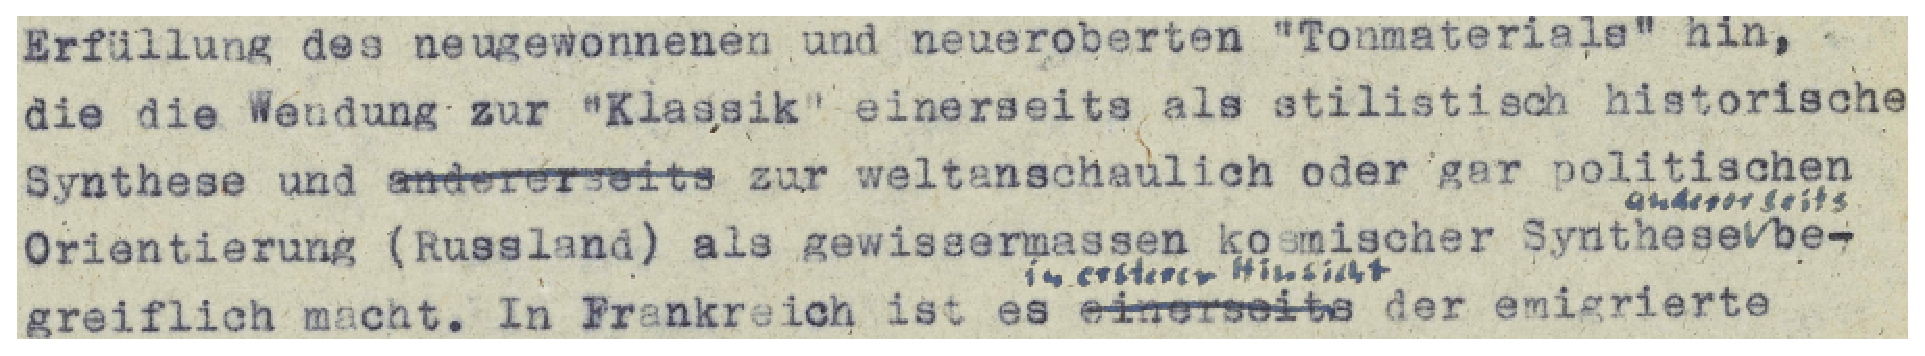
\epsfig{file=figures/ex_typo1.eps,width=\textwidth}
    \begin{tabular}{cc}
      \begin{minipage}{0.3\textwidth}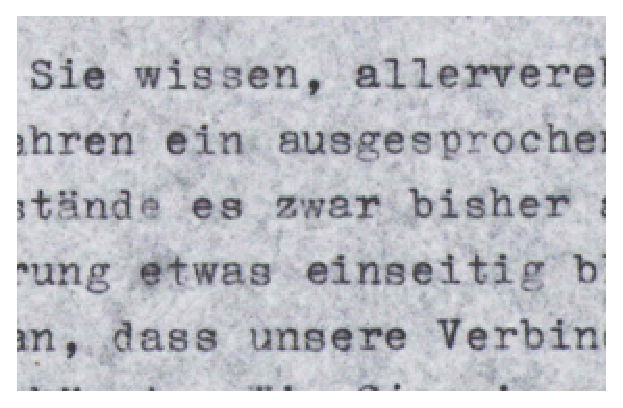
\epsfig{file=figures/ex_typo2.eps,width=\textwidth}\end{minipage}
      &
      \begin{minipage}{0.3\textwidth}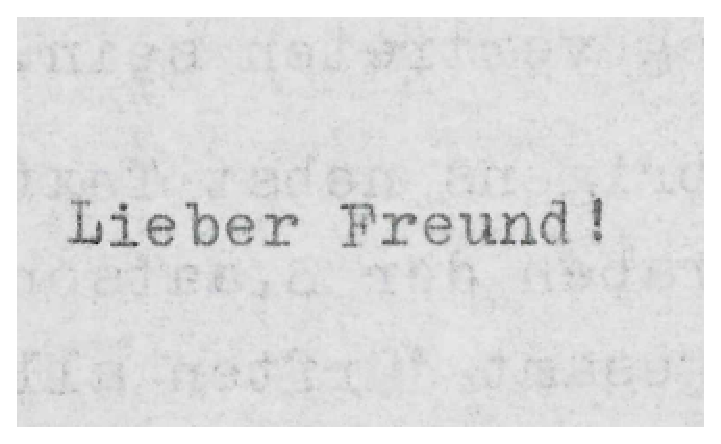
\epsfig{file=figures/ex_typo3.eps,width=\textwidth}\end{minipage}
    \end{tabular}
    \begin{tabular}{cc}
      \begin{minipage}{0.3\textwidth}
\epsfig{file=figures/ex_typo4.eps,width=\textwidth}\end{minipage}
      &
      \begin{minipage}{0.3\textwidth}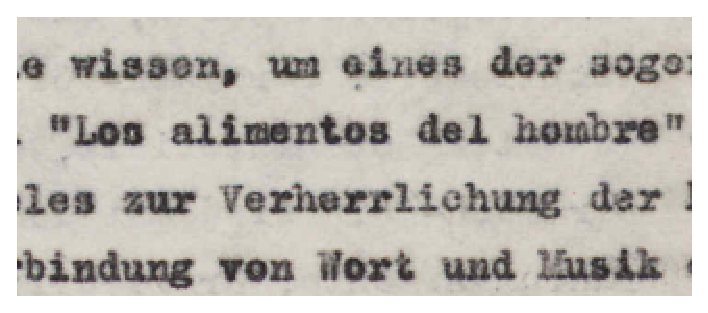
\epsfig{file=figures/ex_typo5.eps,width=\textwidth}\end{minipage}
    \end{tabular}
  \end{center}
\end{bbawslide}

\begin{bbawslide}{Experiment 2: Schreibmaschinentyposkripte}
  \vspace*{4mm}%
  \centerslidestrue%
  \textbf{Vorgehen:}
  \begin{itemize}
    \item manuelle Erfassung von zehn Seiten für Testzwecke (Text plus Layout, aligniert)
    \item Fontauswahl
    \begin{itemize}
      \item riesige Menge an vorhandenen Schriften
      \item teilweise modellspezifisch
      \item mit entsprechenden Artefakten
    \end{itemize}
    \begin{tabular}{cccc}
      \begin{minipage}{0.2\textwidth}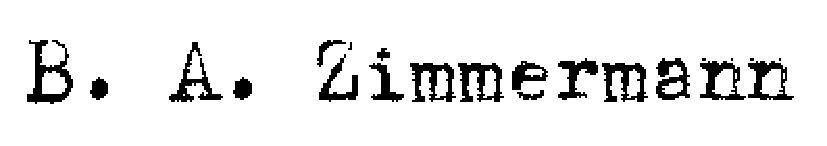
\epsfig{file=figures/ex_underwood.eps,width=\textwidth}\end{minipage}
      &
      \begin{minipage}{0.2\textwidth}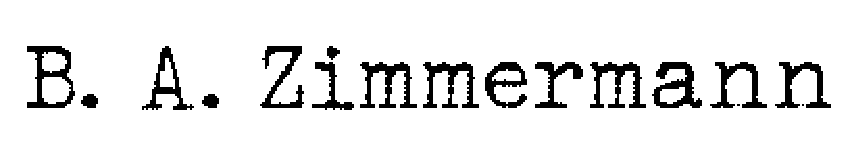
\epsfig{file=figures/ex_rheinmetall.eps,width=\textwidth}\end{minipage}
      &
      \begin{minipage}{0.2\textwidth}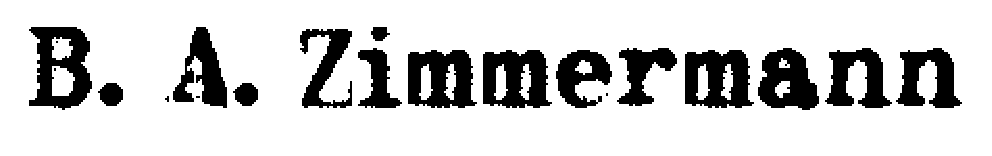
\epsfig{file=figures/ex_byron.eps,width=\textwidth}\end{minipage}
      &
      \begin{minipage}{0.2\textwidth}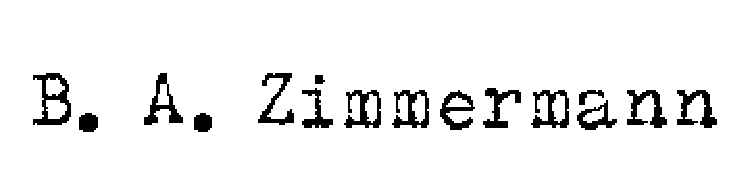
\epsfig{file=figures/ex_olivetti.eps,width=\textwidth}\end{minipage}
      \\
      \small 1913 Underwood No. 5
      &
      \small Rheinmetall 1952
      &
      \small Byron Mark 1
      &
      \small Olivetti Lettera 32
      \\
      \begin{minipage}{0.15\textwidth}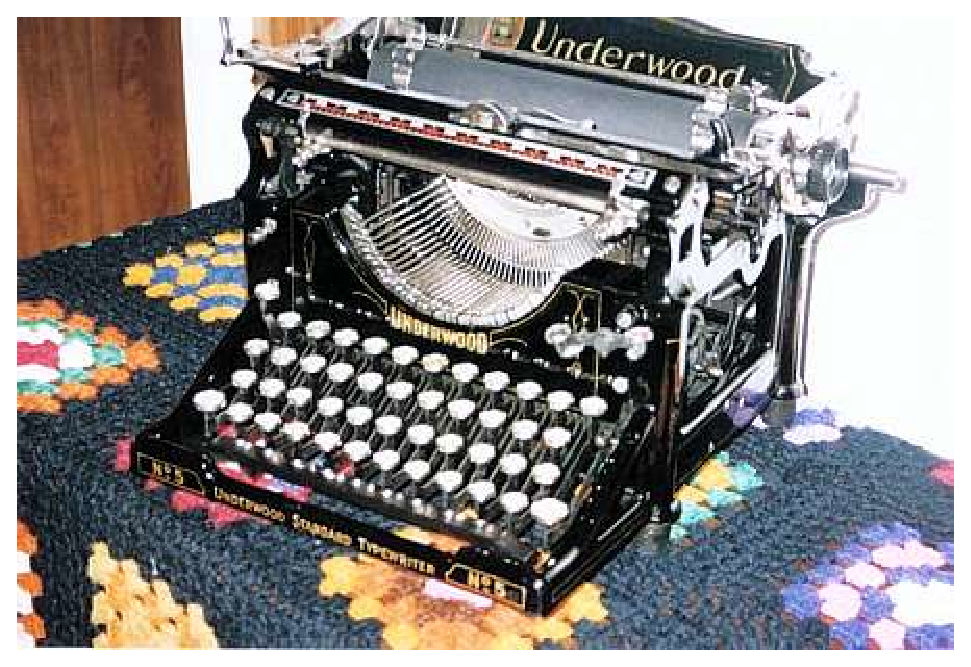
\epsfig{file=figures/tw_underwood.eps,width=\textwidth}\end{minipage}
      &
      \begin{minipage}{0.15\textwidth}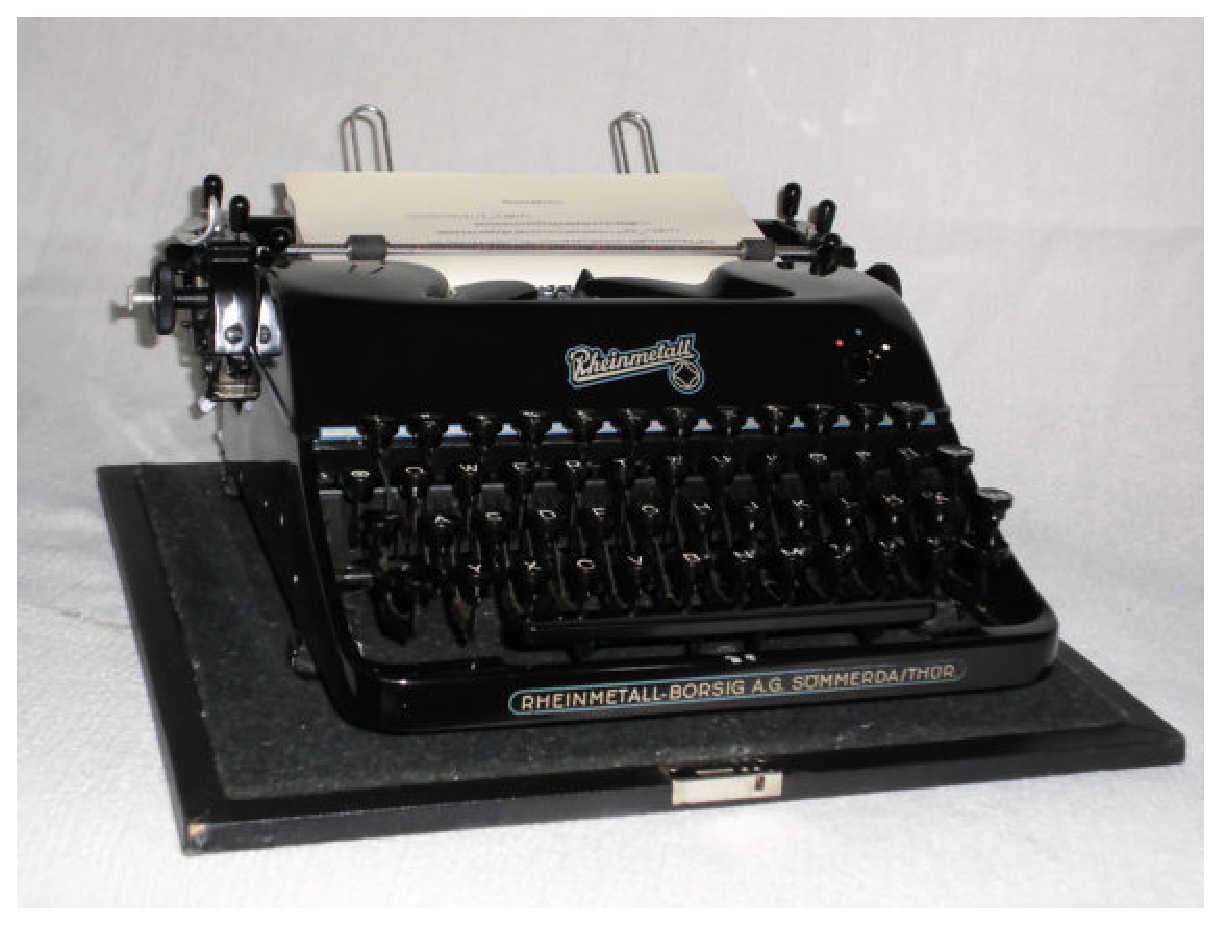
\epsfig{file=figures/tw_rheinmetall.eps,width=\textwidth}\end{minipage}
      &
      \begin{minipage}{0.15\textwidth}\epsfig{file=figures/tw_byron.eps,width=\textwidth}\end{minipage}
      &
      \begin{minipage}{0.15\textwidth}\epsfig{file=figures/tw_olivetti.eps,width=\textwidth}\end{minipage}
    \end{tabular}
  \end{itemize}
\end{bbawslide}

\begin{bbawslide}{Experiment 2: Schreibmaschinentyposkripte}
  \vspace*{7mm}%
  \centerslidestrue%
  \textbf{Vorgehen:}
  \begin{itemize}
    \item Texttauswahl
    \begin{itemize}\small
      \item unklarer Faktor
      \item intuitive Auswahl: Briefe
      \item Jean Paul: \enquote{Dritte Abteilung Briefe}. In: \emph{Jean Pauls Sämtliche Werke. Historisch-kritische Ausgabe}. Abt. 3, Bd. 1. Berlin, 1956.
    \end{itemize}
    \item Rendering mit \texttt{Ketos} (\verb_--_\texttt{legacy}-Degradation)
    \item Training mit \texttt{CLSTM} (Standardparameterbelegung)
    \begin{itemize}\small
      \item nur reales Trainingsmaterial
      \item nur synthetisches Trainingsmaterial
      \item gemischt
    \end{itemize}
  \end{itemize}
\end{bbawslide}

\begin{bbawslide}{Experiment 2: Schreibmaschinentyposkripte}
  \vspace*{7mm}%
  \centerslidestrue%
  \textbf{Ergebnisse:}
  \begin{itemize}
    \item 215 Zeilen reales Trainingsmaterial, 95 Zeilen Testmaterial
    \item jeweils 40000 Trainingsschritte, Auswahl des besten Modells
  \end{itemize}
  \begin{tabular}{lrp{0.5\textwidth}}
    \textbf{Modell} & \textbf{CER} & \textbf{Beschreibung}\\
    \texttt{Abbyy} & 5\,\% & Abbyy FineReader 14\\
    \texttt{Real} & 17\,\% & 17000 Trainingsschritte \\
    \texttt{Synthetic} & 17\,\% \\
    \texttt{Mixed-simple} & 22\,\% & 17000 Trainingsschritte auf ca. 10000 Zeilen \\
    \texttt{Mixed-komplex} & 15\,\% & 26000 Trainingsschritte auf ca. 9000 Zeilen \\
  \end{tabular}
\end{bbawslide}

\begin{bbawpart}{\Large\bf Hypothesen und Lösungsmöglichkeiten}
\end{bbawpart}

\begin{bbawslide}{Hypothesen und Lösungsmöglichkeiten}
  \vspace*{7mm}%
  \centerslidestrue%
  \begin{description}
    \item[\labelitemi] Distanz zwischen synthetischem Trainingsmaterial und realen Daten zu groß
    \item[$\rightarrow$] mehr bzw. realistischere Degradation
    \item[$\rightarrow$] passendere Schriftarten
    \item[$\rightarrow$] realistischeres Rendering (Graustufen oder Farbrendering)
    \item[\labelitemi] Modelle konvergieren zu schnell
    \item[$\rightarrow$] mehr Trainingsdaten, mehr Schriftarten
    \item[$\rightarrow$] alternative Parameterbelegung beim Training
    \item[\labelitemi] Hebräisch: Alphabet zu groß
    \item[$\rightarrow$] getrennte Erkennung von Buchstaben und Diakritika
  \end{description}
\end{bbawslide}

\begin{bbawpart}{\Large\bf Danke für Ihre Aufmerksamkeit!\\}
OCR-D-Team: Elisa Hermann, Maria Federbusch, Clemens Neudecker, Ajinkya Prabhune, \textbf{Matthias Boenig}
\end{bbawpart}

\end{document}

%\begin{bbawpart}{\Large\bf Warum braucht man OCR?}
%\end{bbawpart}

%\begin{bbawslide}{Warum braucht man OCR?}
%  \vspace*{7mm}%
%  \centerslidestrue%
%  \begin{itemize}
%    \item
%  \end{itemize}
%\end{bbawslide}

%
% modelines
%

%%% Local Variables:
%%% mode: LaTeX
%%% coding: utf-8
%%% tab-width: 2
%%% indent-tabs-mode: nil
%%% End:

% vim: set ts=2 sw=2 expandtab :
